% PAKETE UND DOKUMENTKONFIGURATION
\documentclass[11pt, a4paper]{article}

% Encoding für Umlaute
\usepackage[utf8]{inputenc}
\usepackage[T1]{fontenc}

% Silbentrennung
\usepackage[ngerman]{babel}

% erweiterte Matheumgebungen und Formelnummer mit Sectionnummer
\usepackage{amsmath}
\numberwithin{equation}{section}

% Braket Notation
\usepackage{braket}

% zusätzliche mathematische Schriftarten
\usepackage{amsfonts}

% verschiedene mathematische Symbole
\usepackage{amssymb}

% Einheiten setzen z.B. \SI{10}{\kilo\gram\meter\per\second\squared}
% Fehler: \SI{10 +- 0,2e-4}{\metre}
\usepackage{siunitx}
\sisetup{
  output-decimal-marker={,},
  separate-uncertainty
}

% Randbreiten
\usepackage[left=3.5cm,right=3.5cm,top=3cm,bottom=3cm,twoside]{geometry}

% Bilder einfügen
\usepackage{graphicx}

% Verweise innerhalb des Dokuments
\usepackage{hyperref}
\hypersetup{
	colorlinks = true,
	allcolors = {black}
}

% bessere Tabellenlayouts
\usepackage{booktabs}
\usepackage{multirow}

% Seitenlayout (Kopfzeile)
\usepackage{fancyhdr}

% Float Barriers
\usepackage{placeins}

% Pakete für gedrehte Subfigures
\usepackage{caption}
\usepackage{subcaption}
\usepackage{rotating}

% Caption-Setup
\captionsetup{font={small}}
\renewcommand{\thefigure}{\thesection.\arabic{figure}}
\renewcommand{\thesubfigure}{\alph{subfigure}}
\renewcommand{\thetable}{\thesection.\arabic{table}}
\renewcommand{\thesubtable}{\alph{subtable}}

% Manuelle Silbentrennung
\hyphenation{}

% Tiefe des Inhaltsverzeichnisses (Level: 1 sections, 2 subsections,
% 3 subsubsections)
\setcounter{tocdepth}{3}

% FANCYHDR SETUP
\pagestyle{fancy}
\fancyhead[EL,OR]{\thepage}
\fancyhead[ER]{\leftmark}
\fancyhead[OL]{\rightmark}

\renewcommand{\sectionmark}[1]{
\markboth{\thesection{} #1}{\thesection{} #1}
}
\renewcommand{\subsectionmark}[1]{
\markright{\thesubsection{} #1}
}

% DOKUMENTINFORMATIONEN
\title{P442 \\ Laser}

\author{Christopher Deutsch\footnote{christopher.deutsch@uni-bonn.de} \and Christian Bespin\footnote{christian.bespin@uni-bonn.de}}

\date{\today}

\begin{document}

\begin{titlepage}

\maketitle

% DURCHFÜHRUNGSDATUM UND TUTOR
\begin{center}
\begin{tabular}{l r}
Durchführung: & 15./16. Dezember 2014 \\
Gruppe: & $\alpha$ 2 \\
Tutor: & Tobias Macha
\end{tabular}
\end{center}

% ZUSAMMENFASSUNG
\begin{abstract}
\noindent

\end{abstract}

\end{titlepage}

% INHALTSVERZEICHNIS
\tableofcontents
% Neue Seite nach TOC
\newpage

% INHALT VERSUCHSPROTOKOLL

\section{Einführung}

\section{Theorie}

\section{Durchführung und Auswertung}
Sofern nicht anders angegeben Durchführung wie in Praktikumsanleitung.

\subsection{Aufbau des Helium-Neon Experimentierlasers und Charakterisierung der Intensität}

\subsection{Bestimmung der Wellenlänge des Lasers mit einem Reflexionsgitter}
\subsubsection{Durchführung}
\begin{figure}[h]
	\centering
	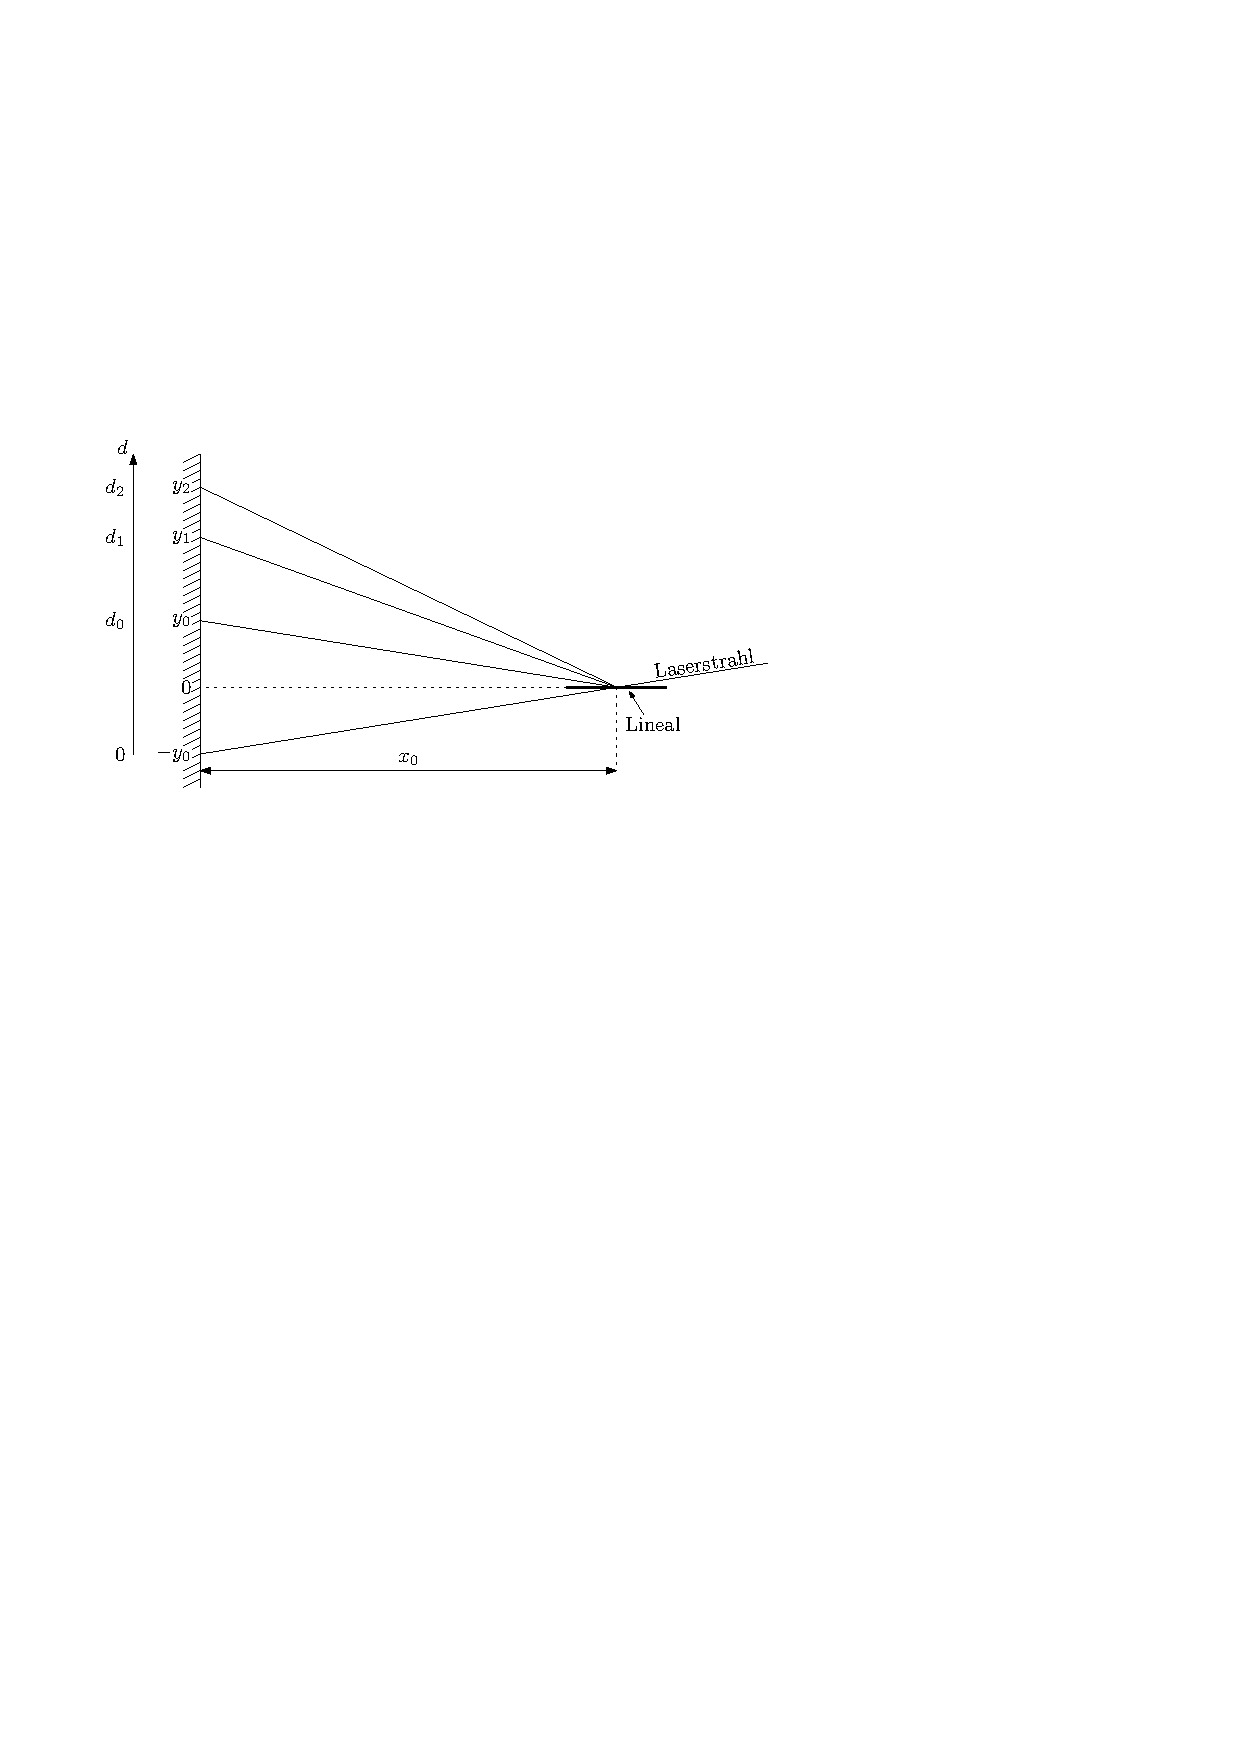
\includegraphics[width=0.9\textwidth]{./figures/wellenlaenge_lineal.pdf}
	\caption{Wellenlängenbestimmung nach Schawlow \cite{schawlow} und die im Versuch gemessenen Längen $d$}
	\label{fig:schawlow}
\end{figure}
Zur Bestimmung der Wellenlänge des Lasers nach Schawlow \cite{schawlow} wird ein Stahlmaßstab mit eingravierter Skaleneinteilung als Reflexionsgitter verwendet.
Dazu wird der Laserstrahl in flachem Winkel auf die Millimeter-Skala des Maßstabes geleitet, sodass ein scharfes Interferenzmuster auf dem Whiteboard in einer Entfernung (von der beleuchteten Stelle Lineal) von $x_0 = \SI{252 +- 2}{\centi\metre}$ entsteht.
Anschließend werden die Maxima des Musters markiert, wobei darauf geachtet werden muss, dass bei der nullten Beugungsordnung begonnen wird, um negative Beugungsordnungen zu vermeiden.
Die nullte Beugungsordnung kann daran erkannt werden, dass sie maximale Intensität aufweist.
Nachdem ausreichend viele Ordnungen markiert wurden, wird das Lineal aus dem Strahlengang entfernt und der Auftreffpunkt des Laserstrahls auf dem Whiteboard markiert.



Identifikation der Reflektion (nullte Beugungsordnung) aufgrund hoher Intensität.


\subsubsection{Auswertung}

Zunächst wird die Position $y_0$ des reflektierten Strahls (nullte Beugungsordnung) auf dem Schirm berechnet durch:
\begin{align}
	y_0 = \frac{d_0}{2} \text{.}
\end{align}
Mit dem gemessenen Wert $d_0 = \SI{19.7 +- 0.2}{\centi\metre}$ kann diese bestimmt werden zu:
\begin{align}
	y_0 = \SI{9.85 +- 0.10}{\centi\metre}
\end{align}
Damit können nun die restlichen Positionen $y_n$ der $n$-ten Beugungsordnungen bestimmt werden durch:
\begin{align}
	y_n &= d_n - y_0 \\
	\Delta y_n &= \sqrt{\Delta d_n^2 + \Delta y_0^2}
\end{align}
Anschließend kann gemäß \cite{schawlow}:
\begin{align}
	\lambda = \frac{g}{2 n} \left( \frac{y_n^2 - y_0^2}{x_0^2} \right)
\end{align}
die Wellenlänge aus den einzelnen Interferenzmaxima berechnet werden, wobei $g$ die Gitterkonstante des Reflexionsgitters bezeichnet.
Unter Vernachlässigung des Fehlers in der Gitterkonstante des Lineals berechnet sich der Fehler aus Gauß'scher Fehlerfortpflanzung zu:
\begin{align}
	\Delta \lambda = \frac{g}{2 n} \sqrt{\left( \frac{2 y_n}{x_0^2} \right)^2 \cdot \Delta y_n^2 + \left( \frac{2 y_0}{x_0^2} \right)^2 \cdot \Delta y_0^2 + \left(\frac{2\left(y_n^2 - y_0^2 \right)}{x_0^3}\right)^2 \cdot \Delta x_0^2}
\end{align}
Mit diesen Überlegungen erhält man die Werte aus Tabelle \ref{tab:wellenlaengen_berechnung}.
\begin{table}[h]
	\centering
	\begin{tabular}{SSSSSSS}
\toprule
{$n$} & {$d_n$ / \si{\centi\metre}} & {$\Delta d_n$ / \si{\centi\metre}} & {$y_n$ / \si{\centi\metre}} & {$\Delta y_n$ / \si{\centi\metre}} & {$\lambda$ / \si{\nano\metre}} & {$\Delta \lambda$ / \si{\nano\metre}} \\
\midrule
1  & 23.2 & 0.2 & 13.35 & 0.23 & 639 & 51 \\
2  & 26.0 & 0.2 & 16.15 & 0.23 & 645 & 32 \\
3  & 28.1 & 0.2 & 18.25 & 0.23 & 619 & 25 \\
4  & 30.2 & 0.2 & 20.35 & 0.23 & 624 & 21 \\
5  & 32.0 & 0.2 & 22.15 & 0.23 & 620 & 19 \\
6  & 34.0 & 0.2 & 24.15 & 0.23 & 638 & 18 \\
7  & 35.4 & 0.2 & 25.55 & 0.23 & 625 & 17 \\
8  & 37.1 & 0.2 & 27.25 & 0.23 & 635 & 16 \\
9  & 38.5 & 0.2 & 28.65 & 0.23 & 633 & 16 \\
10 & 39.7 & 0.2 & 29.85 & 0.23 & 625 & 15 \\
11 & 41.3 & 0.2 & 31.45 & 0.23 & 639 & 15 \\
12 & 42.4 & 0.2 & 32.55 & 0.23 & 632 & 14 \\
13 & 43.5 & 0.2 & 33.65 & 0.23 & 627 & 14 \\
14 & 44.8 & 0.2 & 34.95 & 0.23 & 632 & 14 \\
15 & 46.0 & 0.2 & 36.15 & 0.23 & 635 & 14 \\
16 & 47.1 & 0.2 & 37.25 & 0.23 & 635 & 14 \\
17 & 47.9 & 0.2 & 38.05 & 0.23 & 626 & 13 \\
18 & 49.2 & 0.2 & 39.35 & 0.23 & 635 & 13 \\
19 & 50.4 & 0.2 & 40.55 & 0.23 & 641 & 13 \\
\bottomrule
\end{tabular}
	\caption{Messdaten und Berechnung zur Wellenlängenbestimmung}
	\label{tab:wellenlaengen_berechnung}
\end{table}
Es wird der varianzgewichtete Mittelwert:
\begin{align}
	\bar{\lambda} = \frac{\sum_i \frac{\lambda_i}{\Delta \lambda_i^2}}{\sum_i \frac{1}{\Delta \lambda_i^2}}
\end{align}
wobei der Fehler des Mittelwerts
\begin{align}
\Delta \bar{\lambda} = \frac{1}{\sqrt{\sum_i \frac{1}{\Delta \lambda_i^2}}}
\end{align}
somit folgt:
\begin{align}
	\bar{\lambda} = \SI{632.0 +- 3.6}{\nano\metre}
\end{align}

\subsubsection{Vergleich mit der exakten Rechnung}


\subsection{Untersuchung der Polarisation des Lasers}

Zur Untersuchung der Polarisation des hier verwendeten Experimentierlasers wird der Intensitätsverlauf an einer Photodiode in Abhängigkeit des Winkels eines davor stehenden Linearpolarisators betrachtet.
Dieser ist in der Lage, einfallendes Licht in eine vorgegebene Richtung linear zu polarisieren.
Für den Fall, dass das einfallende Licht bereits linear polarisiert ist (wie für den hier verwendeten Laser angenommen werden kann), gilt für die hinter dem Polarisator registrierte Intensität (Gesetz von Malus):
\begin{align}
I=I_0\cdot\cos^2\varphi
\end{align}

\subsection{Messung des Strahlprofils und des Stabilitätsgebiets des Lasers}

\subsection{Aufbau der optischen Diode}

\subsection{Optischer Spektrumanalysator}

\subsection{Präzise Messung des Modenabstandes mittels einer optischen Schwebung}

\section{Fazit}


% BIBLIOGRAPHIE
\vspace{\fill}
% Maximale Anzahl der Einträge in Klammer
% Zitieren mit \cite{lamport94}
\begin{thebibliography}{9}
\bibitem{schawlow}
	A. L. Schawlow,
	\emph{Measuring the Wavelength of Light with a Ruler},
	Am. J. Phys., Volume 33, Issue 11 (1965)
 
\end{thebibliography}

\clearpage

% APPENDIX
\begin{appendix}
\section{Anhang}


\end{appendix}

\end{document}
